\chapter{Experimentaci\'on y Resultados}\label{chapter:experiments}
En este cap\'itulo se evaluan los resultados obtenidos por AutoGOAL Multiobjetivo tras aplicarse sobre tres corpus de datos utilizando los pares de m\'etricas precis\'on contra recobrado y \textit{f-score} contra tiempo de entrenamiento:
\begin{itemize}
    \item Precisi\'on es una m\'etrica que mide las muestras clasificadas correctamente entre todas las muestras extra\'idas.
    \item Recobrado mide las muestras clasificadas correctamente sobre todas las extra\'idas.
    \item \textit{F-score} es el promedio harm\'onico entre precisi\'on y recobrado.
    \item \textit{Tiempo de entrenamiento} es un estimado que mide cuanto tiempo toma para una flujo de Aprendizaje Autom\'atico en realizar el proceso de entrenamiento.
\end{itemize}

Se utiliza el par de metricas precisi\'on y recobrado pues son crietrios que pueden tener comportamientos variados. Existen problemas donde es posble maximizar ambas y otros donde es obligatorio realizar consesiones entre estas tal que no exista una mejor soluci\'on sino un conjutno de estas.

Se utilza \textit{f-score} contra tiempo de entrenamiento para probar si es posible dirigir efectivamente  la b\'usqueda maximizando la relevancia y minimizando el tiempo de ejecuci\'on. Es posible utilzar tambi\'en precisi\'on y recobrado junto con tiempo de entrenamiento pero con el objetivo de mantener estos primeros experimentos m\'as sencillos se utiliza \textit{f-score}.

\section{Corpus de Evaluaci\'on}
Se utilizan tres corpus de datos para comprobar el comportamiento del sistema cuando optmiza para varias m\'etricas simult\'aneamente. Los corpus se escogen de distintos tamaños y cada uno representa versiones distintas del problema de aprendizaje supervisado.

\subsection{CARS}
Cars es un corpus que representa un conjunto de carros con ciertas caracter\'isticas cat\'alogadas cualitativamente (ver \ref{implementation:table:cars:attributes}). El objetivo con este corpus es aprender a clasificar los carros de  acuerdo a sus atributos  en inaceptable, aceptable, bueno o muy bueno (\ref{implementation:table:cars:classes}). El dataset no tiene valores desconocidos.

\begin{table}[ht]
    \centering
    \parbox{.45\linewidth}{
    \begin{tabular} { |l|c| }
        \hline
        Atributos & Valores \\
        \hline
        \hline
        buying & v-high, hihg, med, low \\
        \hline
        maintance &  v-high, hihg, med, low\\
        \hline
        doors & 2, 3, 4, 5-more\\
        \hline
        persons & 2, 4, more\\
        \hline
        lug\_boot & small, med, big\\
        \hline
        safety & low, med, high\\
        \hline
    \end{tabular}
    \caption{Tipos de Atributos en Cars}
    \label{implementation:table:cars:attributes}
    }
    \qquad
    \parbox[t]{.45\linewidth}{
    \begin{tabular} {|l|c|c|}
        \hline
        Clases & N & \% \\
        \hline
        \hline
        unacc & 1210 & 70.023\%\\
        \hline
        acc & 384 & 22.222\%\\
        \hline
        good & 69 & 3.993\%\\
        \hline
        v-good & 65 & 3.762\%\\
        \hline
    \end{tabular}
    \caption{Distribuci\'on de clases en Cars}
    \label{implementation:table:cars:classes}
    }
\end{table}

\subsection{HAHA}
Humor Analysis based on Human Annotation (HAHA), un conjunto de datos que contiene \textit{tweets} en espa\~nol en texto plano codificado en utf-8. Se quiere construir un clasificador que pueda catalogarlos correctamente entre si son humor\'isticos o no. Contiene un total de 30000 tweets donde se utilizan 24000 para entrenaiento y 6000 para evaluaci\'on.

\begin{table}[ht]
    \centering
    \begin{tabular} {|l||c|c|c|}
        \hline
        & Entrenamiento & Evaluaci\'on & Total \\
        \hline
        \hline
        Tweets & 24000 & 6000 & $30000$\\
        \hline
        Graciosos & 9253 & 2342 & 11595\\
        \hline
        No graciosos & 14 757 & 3 658 & 18 405\\
        \hline
        Puntuaci\'on Promedio & 1305 & 275 & 1580\\
        \hline
    \end{tabular}
    \caption{Distribuci\'on de clases en HAHA}
    \label{implementation:table:haha}
\end{table}

\subsection{MEDDOCAN}

Una colecci\'on de 1000 casos cl\'inicos y sus anotaciones PHI. Cada uno est\'a conformado con aproximadamente de 33 oraciones o 495 palabras. Los caso cl\'inico est\'an codificados en texto plano en utf-8 y las anotaciones est\'an en formato BRAT. El objetivo es predecir dichas anotaciones.

\section{Hardware}
 Los experimentos fueron ejecutados en un equipo con las siguientes propiedades: CPU AMD R5 3550h y 32 GB de RAM.

\section{Resultados y An\'alisis}

A continuaci\'on se muestran los resultados obtenidos tras aplicar AutoGOAL Multiobjetivo a los distintos corpus. En las gr\'aficas solo se tiene en cuenta la puntuaci\'on de relevancia obtenida durante entrenamiento y no con respecto a los datos de prueba. Los puntos  grises marcan las mejores soluciones encontradas en cada generaci\'on.  La tonalidad de los puntos var\'ia de acuerdo en que iteraci\'on del algoritmo fue encontrado; a medida que avanzan las generaciones estos se oscurecen. Los puntos marcados con cruces rojas representan las mejores soluciones encontradas por el algoritmo y conforman una aproximaci\'on del frente de Pareto.

En cada conjunto de datos se utilizaron param\'etros distintos debido fundamentalmene a que cada corpus representa problemas con diferente complejidad y cantidad de datos.

\subsection{Cars}
La aplicaci\'on de AutoGOAL en Cars utilza una poblaci\'on total de 40 individuos por generaci\'on, 1 hora de tiempo m\'aximo y 10 segundos de tiempo l\'imite por \textit{pipeline}. Se utilizaron las implementaciones de \textit{f-score}, \textit{precision} y \textit{recall} de Scikit-Learn (\cite{pedregosa2011scikit}) con el promedio \textit{weighted} utilizado para problemas de clasificaci\'on multiclase que pueden tener un desbalance en las clases existentes.

\subsubsection{F-Score contra Tiempo de Entrenamiento}
El resultado, mostrado en la figura \ref{impl:fig:cars:fscore_vs_time}, parece tener un aparente frente con lo que parece que es una forma c\'oncava y  bien distribuida.  El sistema encuentra m\'ultiples soluciones   casi todas con muy buen \textit{f-score} y estas tienen distintos tiempos de entrenamiento, desde los milisegundos hasta un segundo completo. La mayor\'ia de las soluciones se encuentran mayormente acumuladas en los puntos donde se maximiza lo m\'as posible ambas m\'etricas.

\begin{figure}[ht]
    \centering
    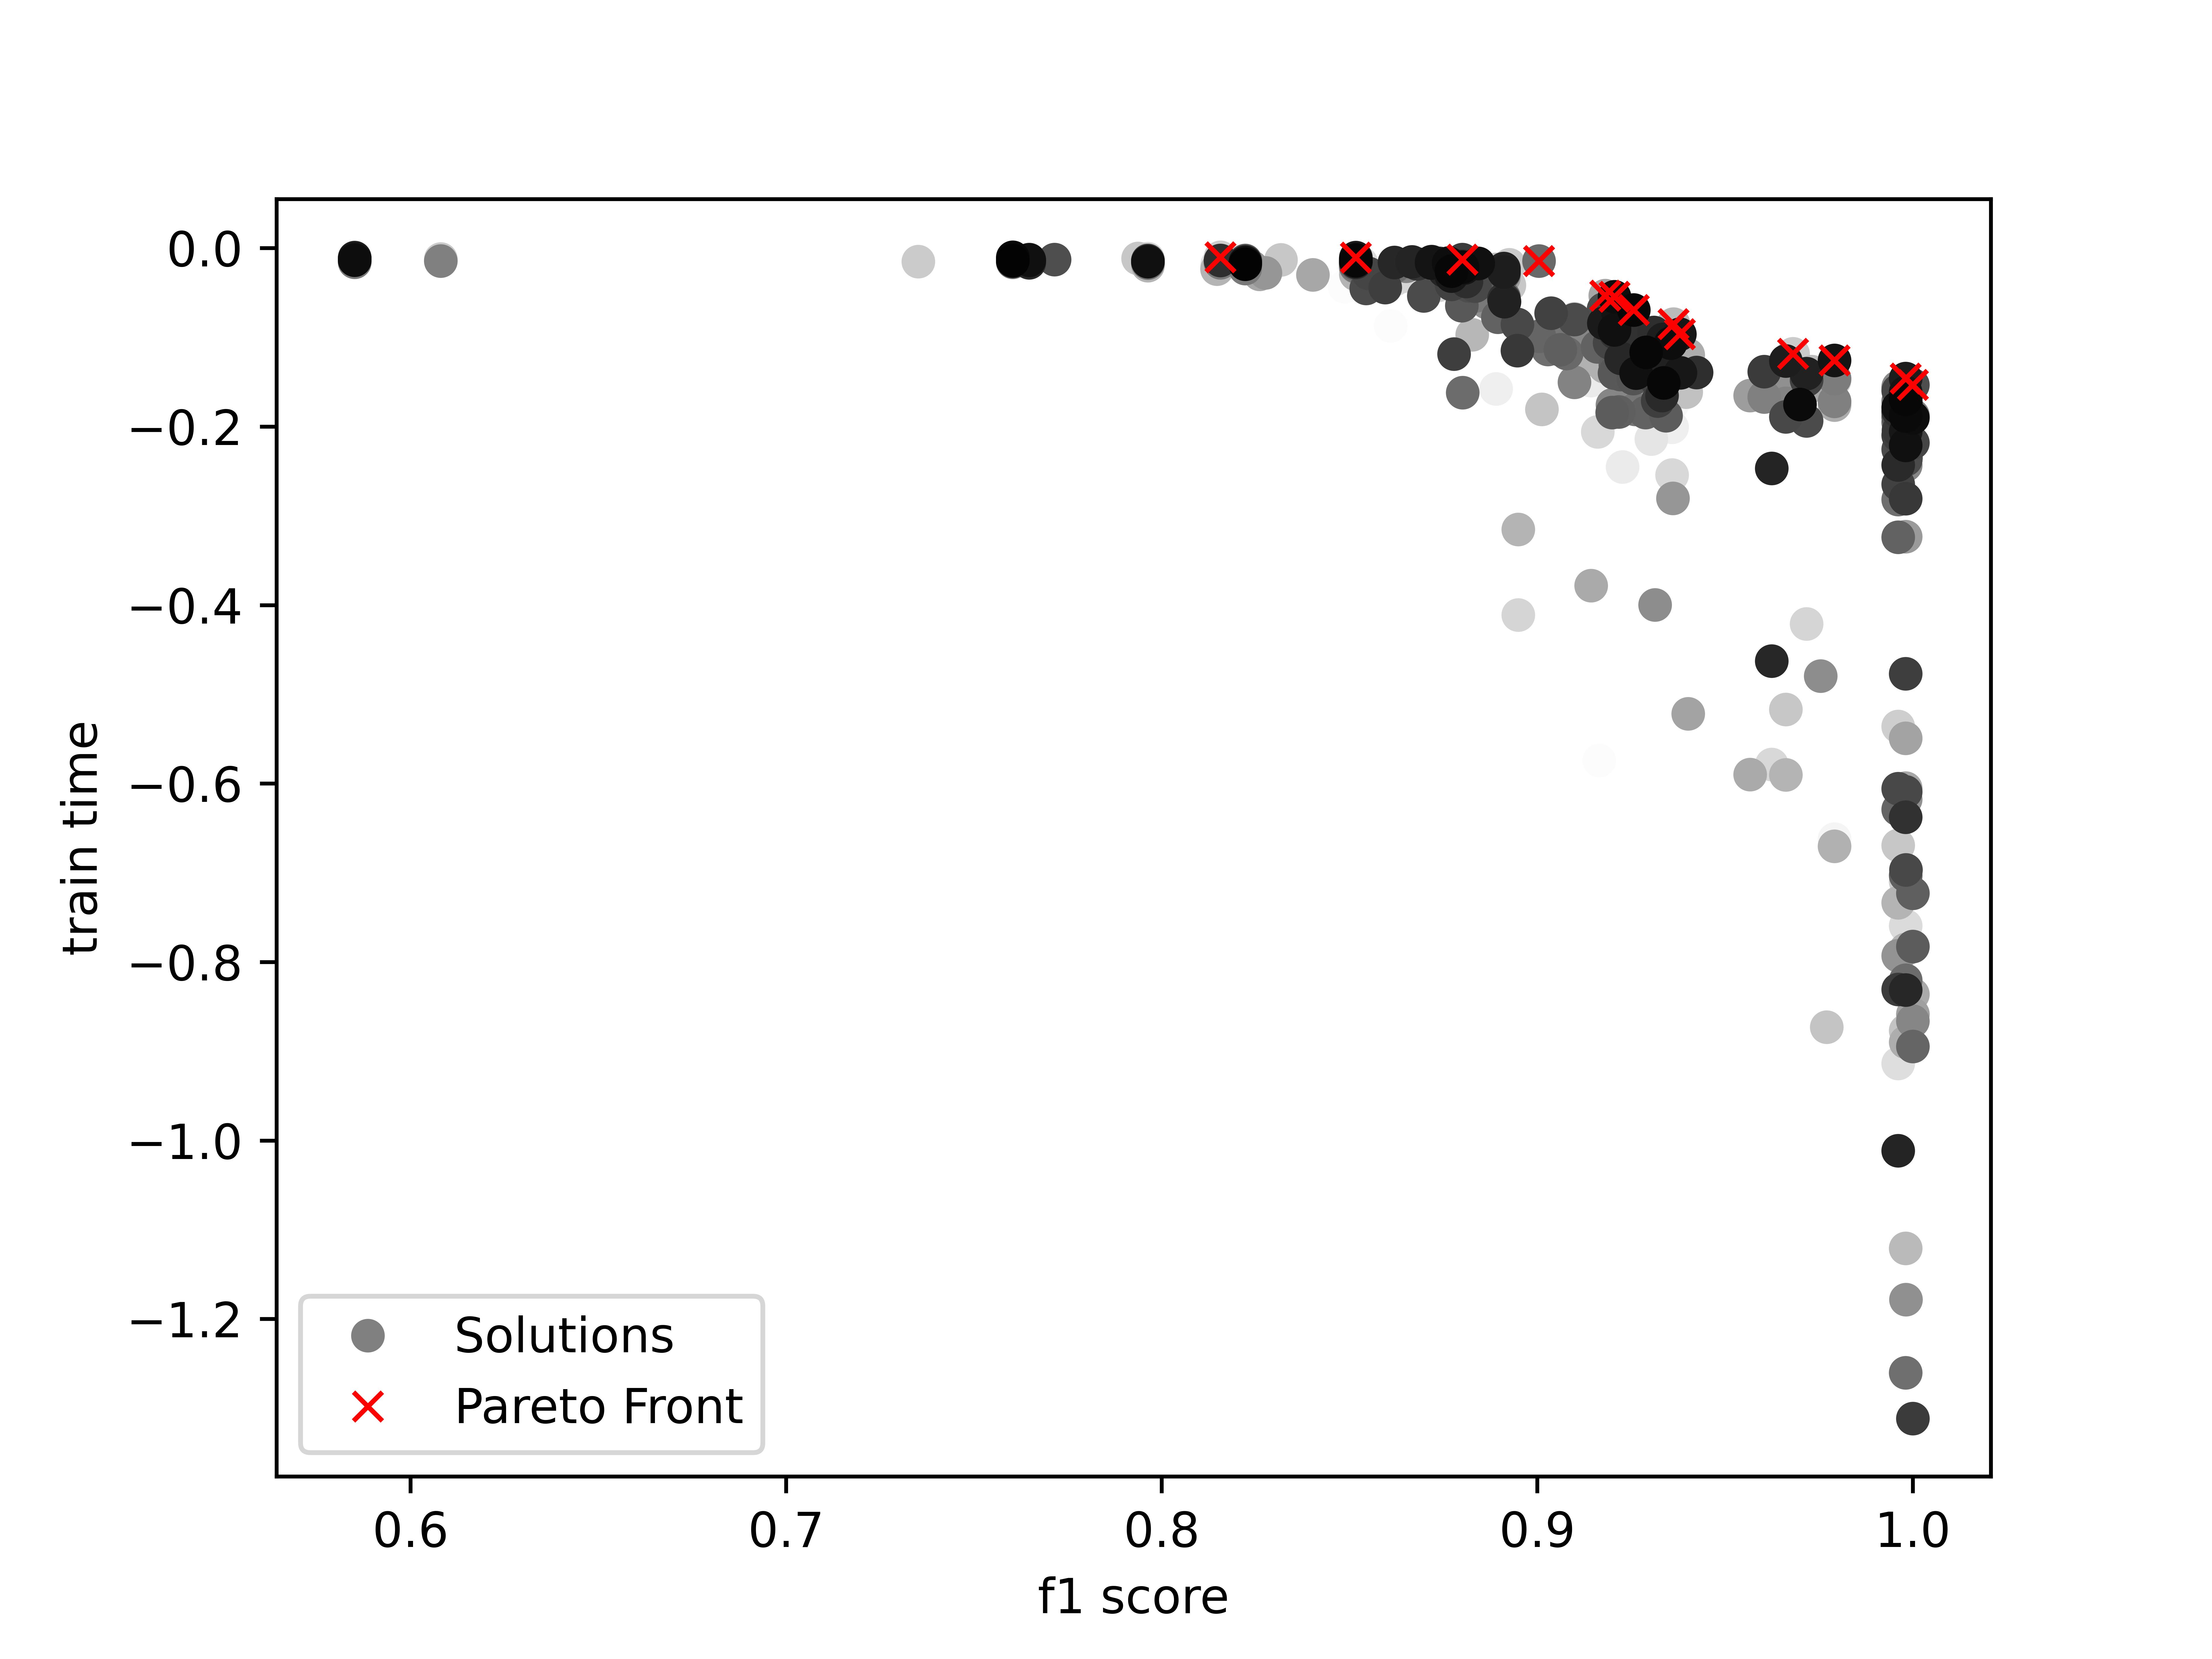
\includegraphics[scale=0.65]{Pictures/cars_fscore_vs_time.jpg}
    \caption{Cars: F-score contra Tiempo de Entrenamiento}
    \label{impl:fig:cars:fscore_vs_time}
\end{figure}


\subsubsection{Precisi\'on contra Recobrado}
Durante esta prueba ocurre un hecho interesante, ni precisi\'on ni recobrado entr\'an en conflicto y por tanto no es necesario hacer concesiones entre una o la otra durante la optimizaci\'on. Se puede observar observa en la figura \ref{impl:fig:cars:precision_vs_recall} que el frente de Pareto esta consituido por un s\'olo punto donde se maximizan precision y recobrado. Tambi\'en se nota como las soluciones van mejorando con el transcurso de las iteraciones.
Adem\'as AutoGOAL encontr\'o 30 soluciones distintas con respecto a algoritmos e hyperpar\'ametros que logran este rendimiento y podr\'ia ser interesante para el investigador analizar las diferencias entre estas.

\begin{figure}[ht]
    \centering
    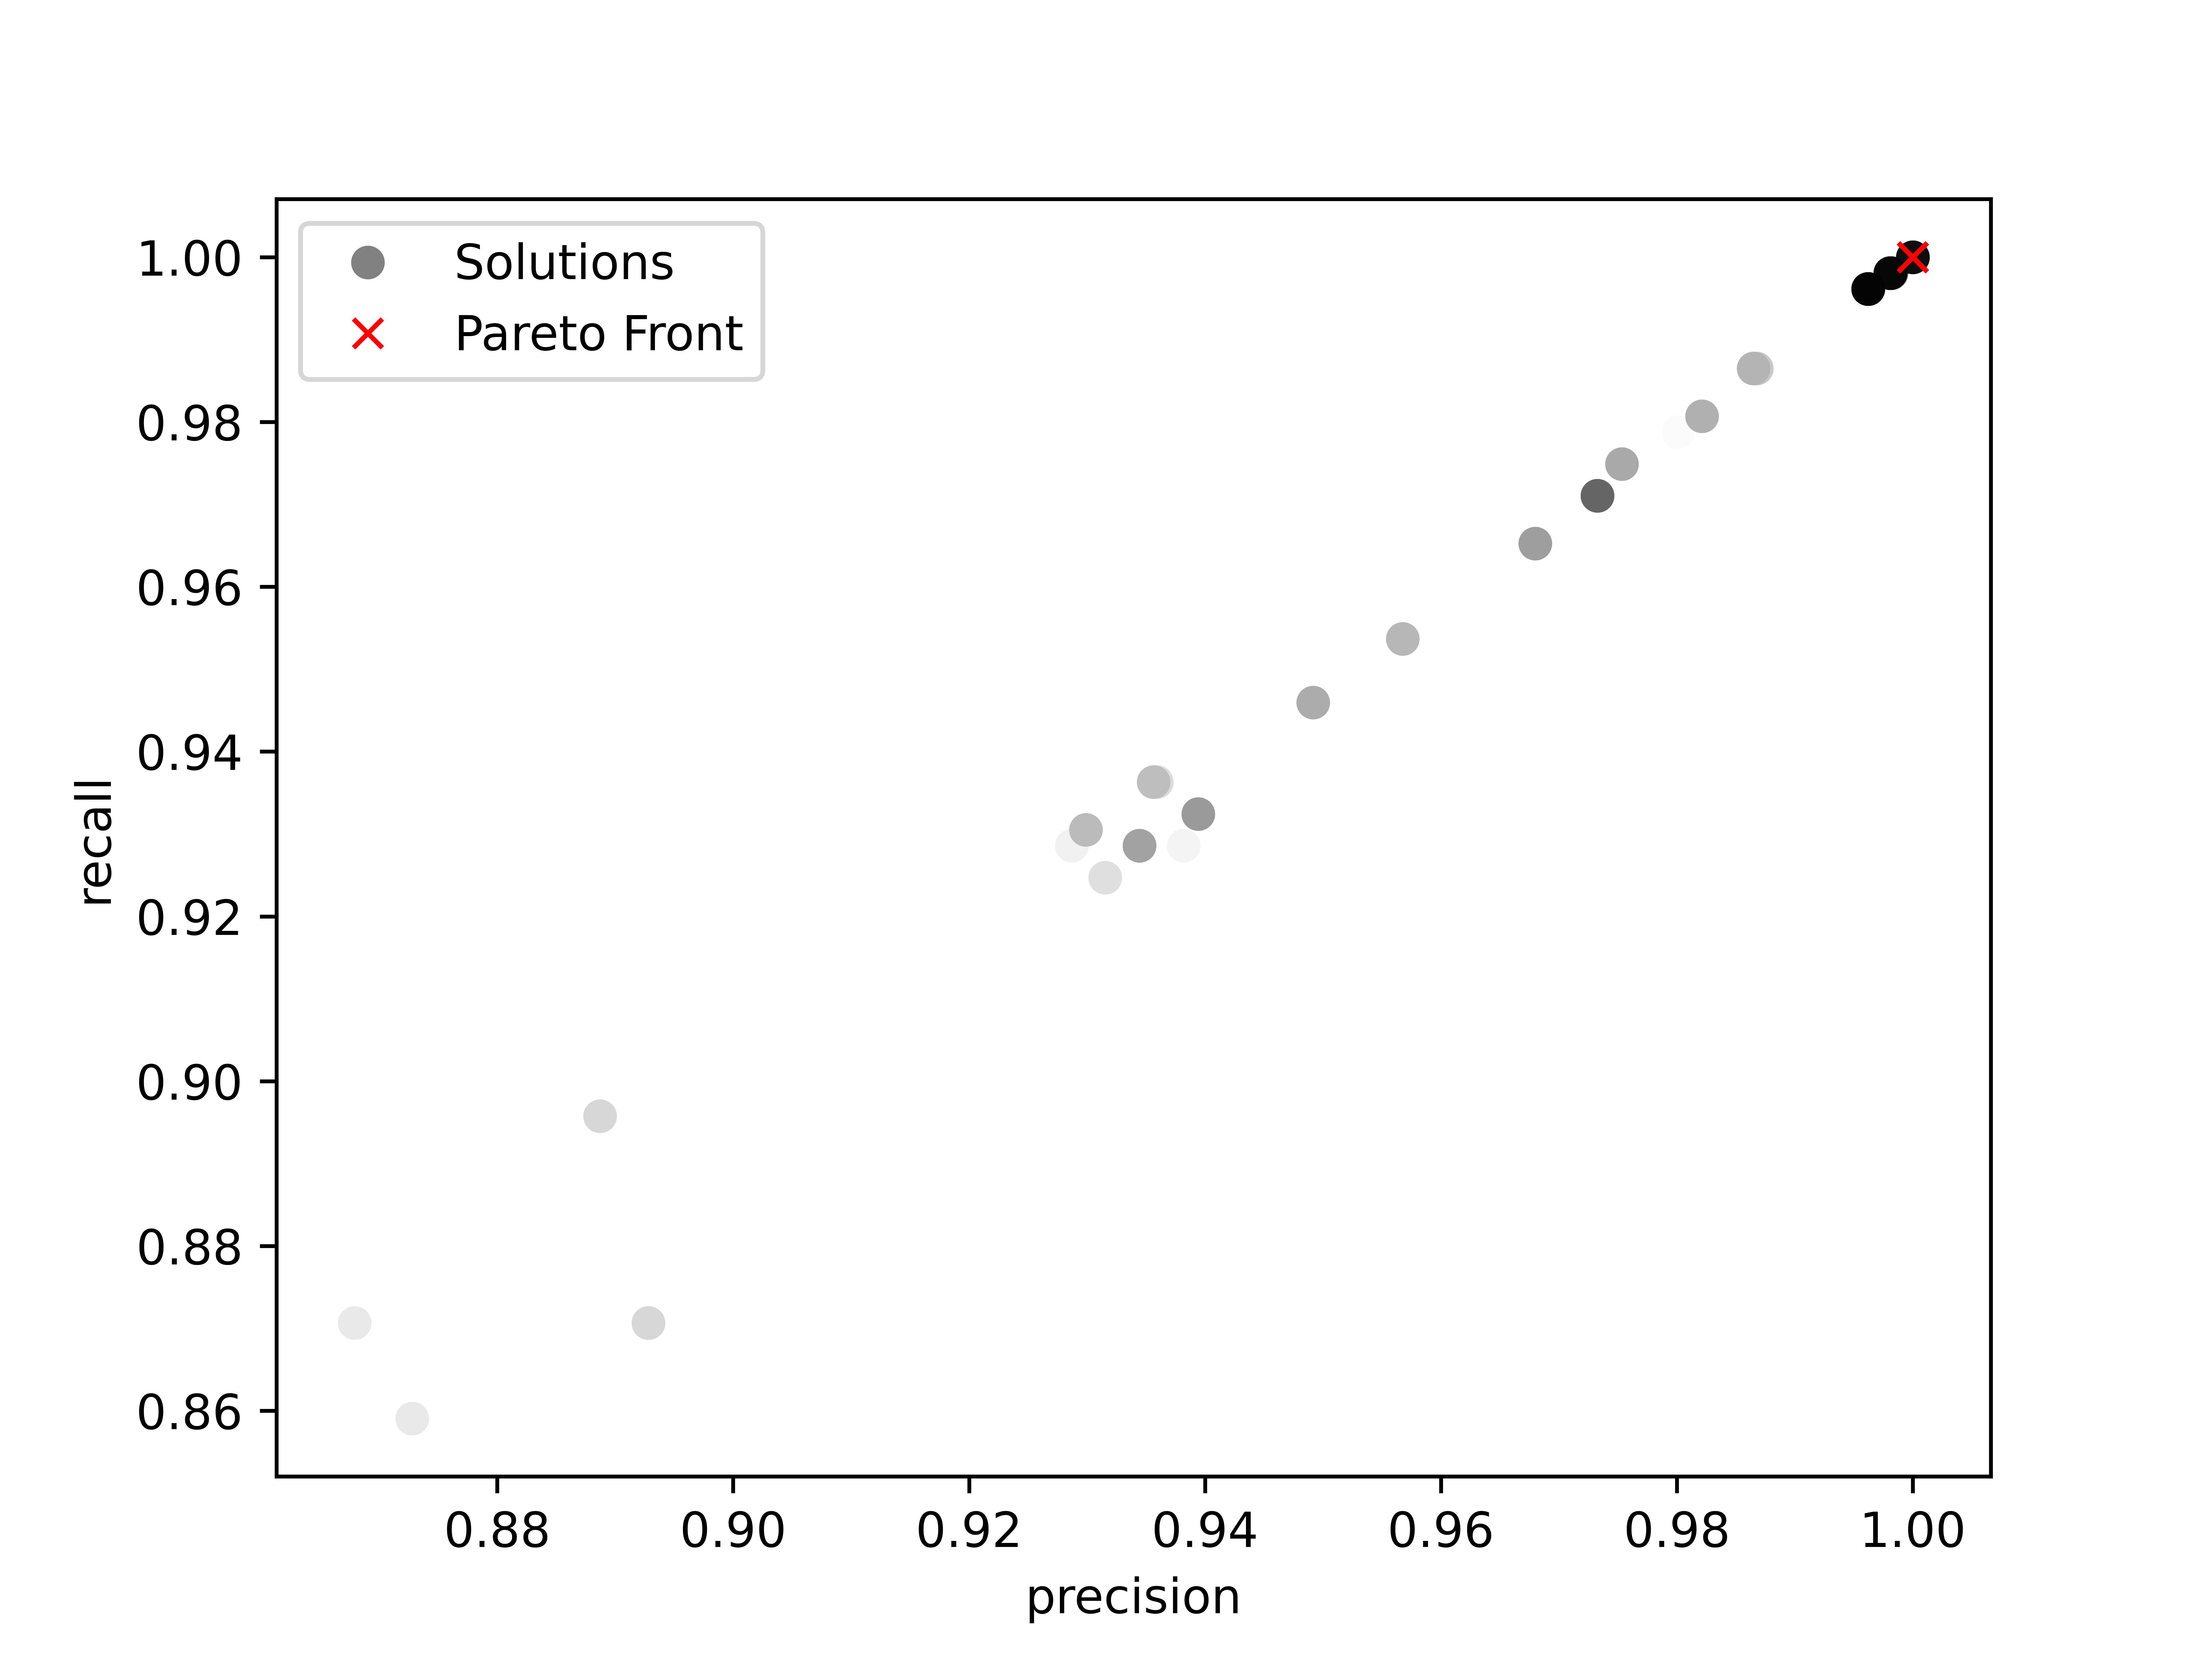
\includegraphics[scale=0.65]{Pictures/cars_precision_vs_recall.jpg}
    \caption{Cars: Precisi\'on contra Recobrado}
    \label{impl:fig:cars:precision_vs_recall}
\end{figure}

\subsection{HAHA}
Se utilzo una poblaci\'on total de 40 individuos, 8 horas de tiempo m\'aximo y 10 segundos por  evaluaci\'on. 
HAHA es un problema de clasificaci\'on binario y las m\'etricas \textit{f-score}, precisi\'on y recobrado son las implementadas en Scikit-Learn (\cite{pedregosa2011scikit}) utilizando promedio binario.

\subsubsection{F-Score contra Tiempo de Entrenamiento}

En esta prueba el frente como se observa en la figura \ref{impl:fig:haha:fscore_vs_time} posee una forma aparentemente similar a \ref{impl:fig:cars:fscore_vs_time}. 

Los soluciones de AutoGOAL en esta experimento est\'an conformados por dos algoritmos principales. Los que contienen poca precisi\'on pero son m\'as rapidos est\'an conformados utilizando t\'ecnicas de \textit{HashingVectorizer} y \textit{NearestCentroid} con variaciones en los hiperpar\'ametros.
Los que tienen mayor precision a costo de un poco de tiempo est\'an compuestos por \textit{CountVectorizer}  y regresores log\'isticos.

Adem\'as en la esquina superior izquierda se ve como AutoGOAL busca un punto que tiene f-score 0, una soluci\'on completamente in\'util y donde se desperdicia tiempo de c\'omputo pero el sistema es agn\'ostico a esto. Una posible mitigaci\'on a esto es definir las m\'etricas aprovechando el mecanismo de AutoGOAL para se\~nalar soluciones incorrectas como: \textit{if f-score} $== 0 \rightarrow $ \textit{retorna} $-\infty$. Esta manera ofrece a\'un m\'as control al usuario sobre el espacio de b\'usqueda pues puede definir dentro de la m\'etrica regiones del espacio objetivo que no le interesen. 


\begin{figure}[ht]
    \centering
    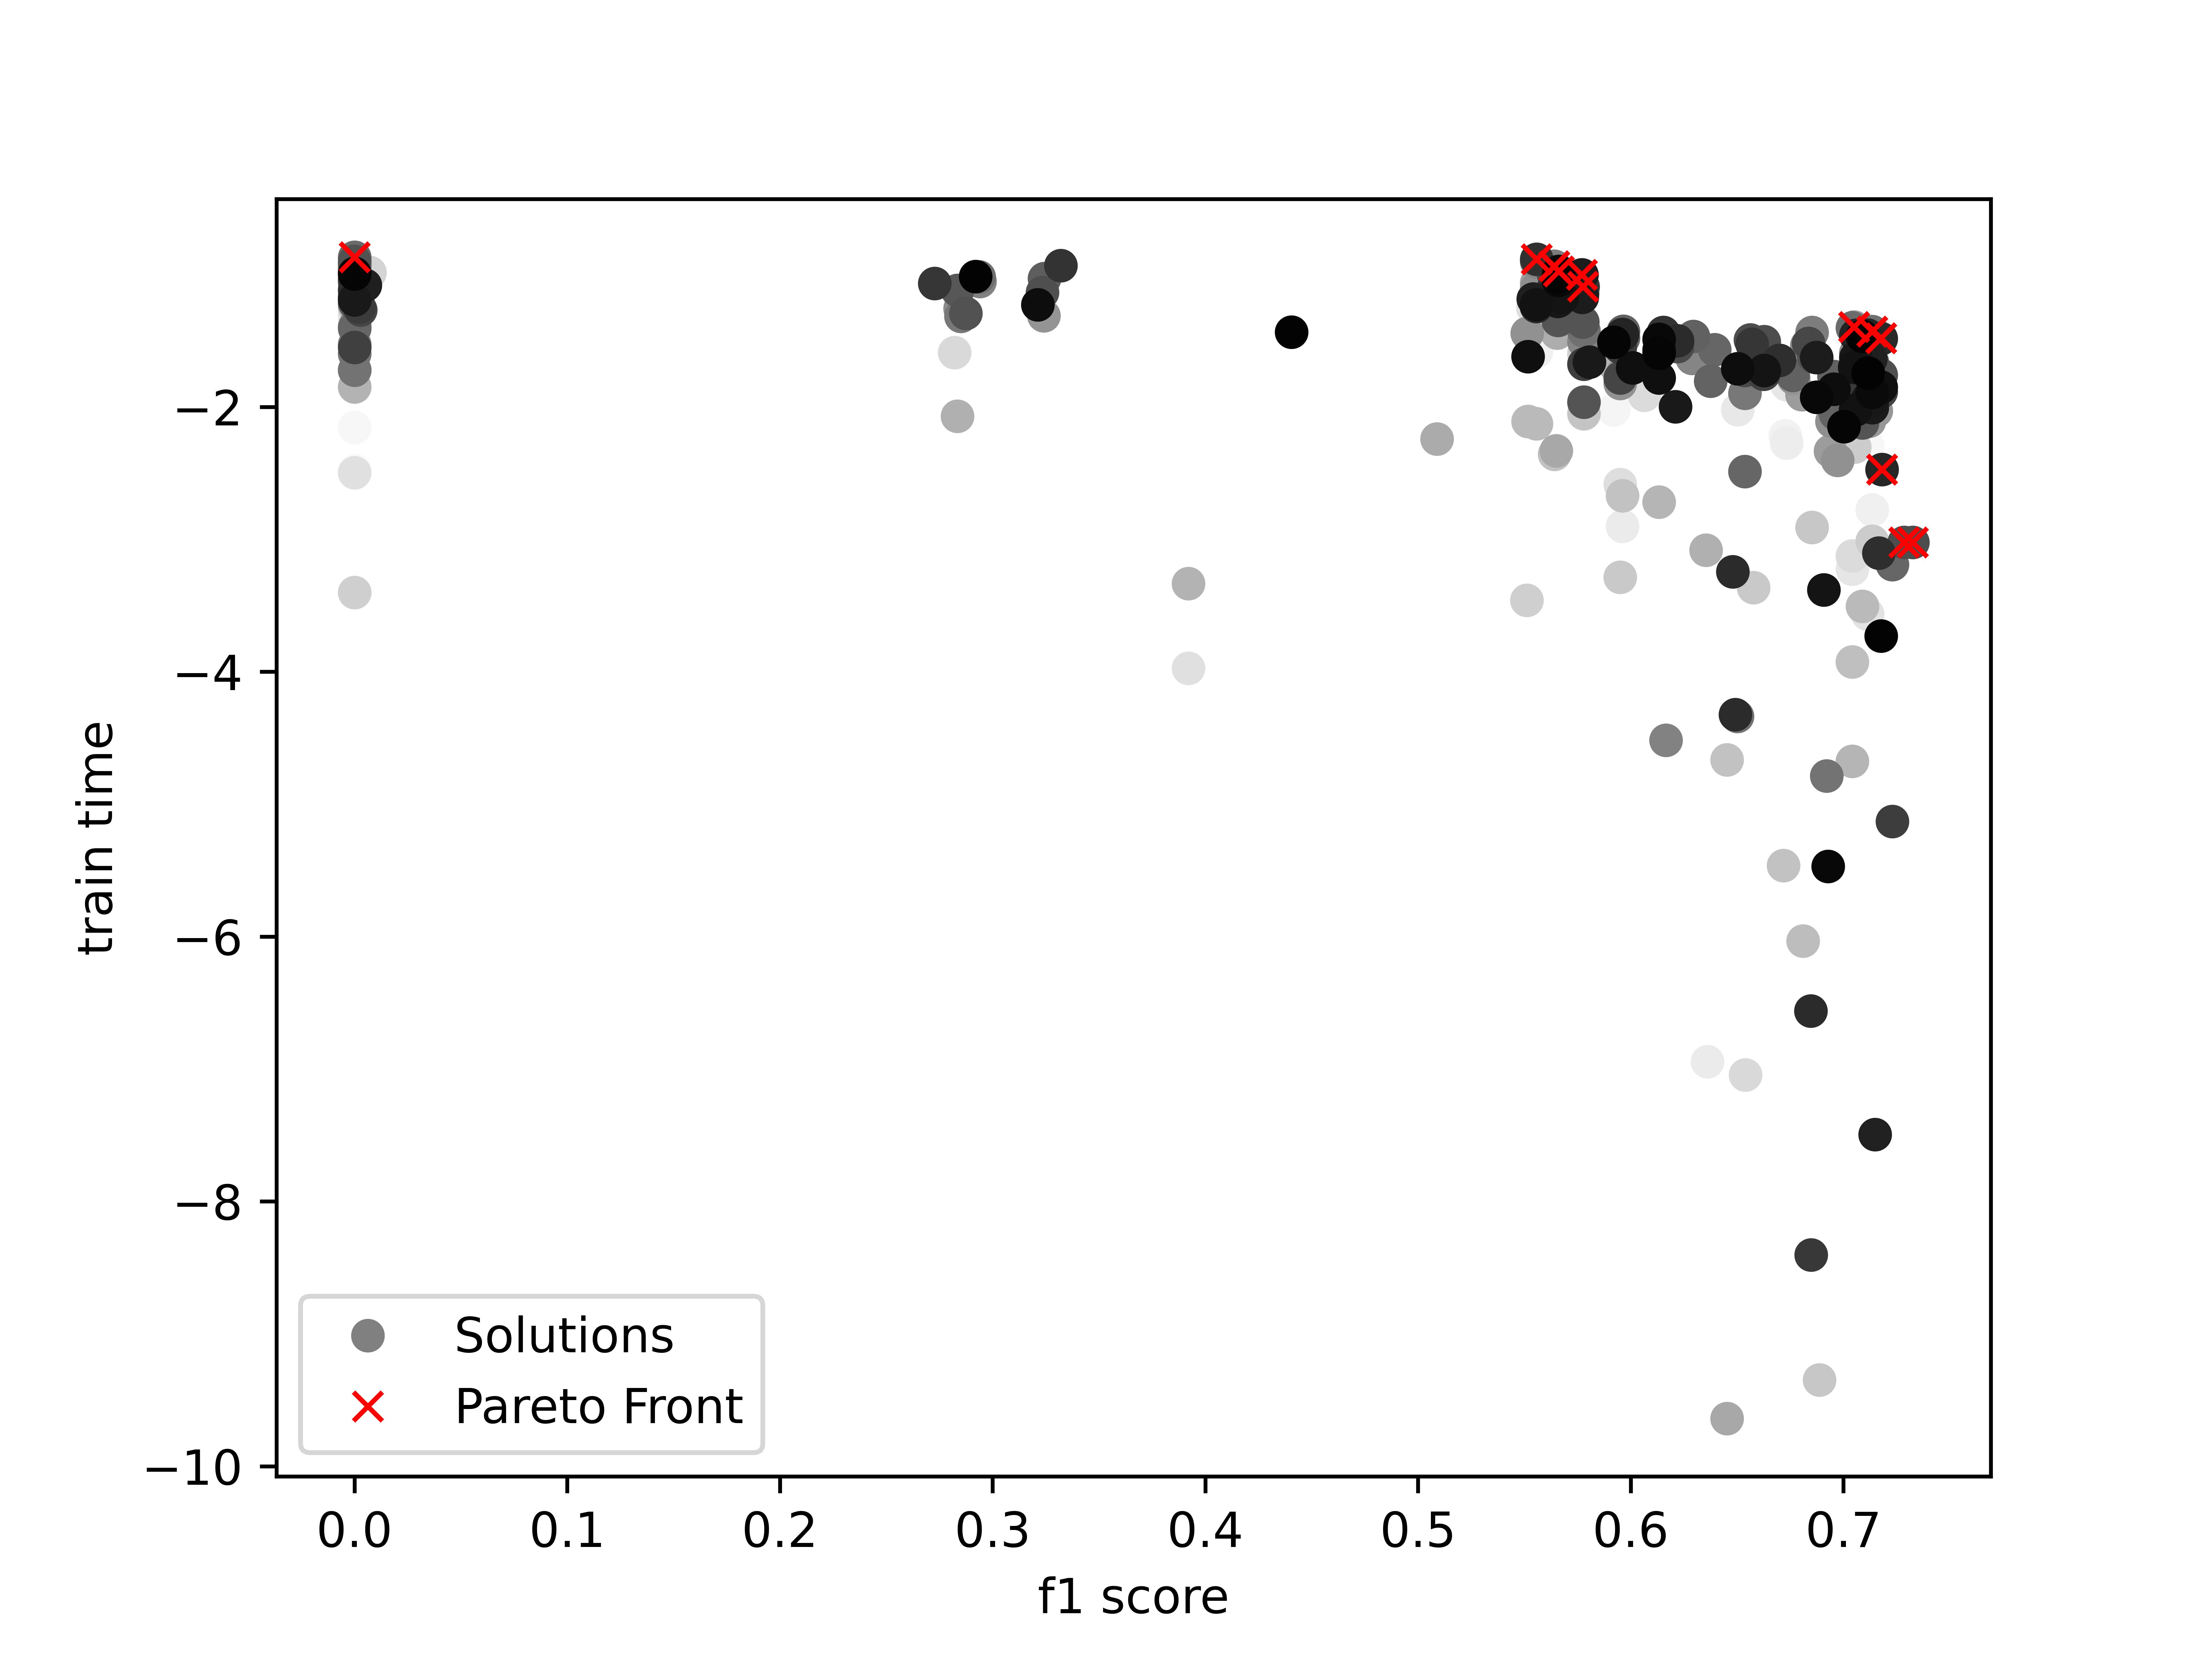
\includegraphics[scale=0.65]{Pictures/haha_fscore_vs_time.jpg}
    \caption{HAHA: F-score contra Tiempo de Entrenamiento (10 segundos m\'ax)}
    \label{impl:fig:haha:fscore_vs_time}
\end{figure}

Otra de las cosas a notar es que hay algoritmos que toman 10 segundos para ejecutarse y posiblemente las soluciones del sistema se vean l\'imitadas por el tiempo m\'aximo asignado a cada \textit{pipeline}. Se realiza una segunda prueba extendiendo esta restricci\'on hasta 3 minutos con el fin de verificar si aumentando el espacio de b\'usqueda se puede obtener una representaci\'on distinta del frente de Pareto. En este caso la estructura extra\~na del frente se mantiene excepto por la aparici\'on de una nueva soluci\'on que destaca sobre el resto donde se obtiene un \textit{f-score} cercano a 0.8 pero con un tiempo de entrenamiento de 30 segundos.

\begin{figure}[ht]
    \centering
    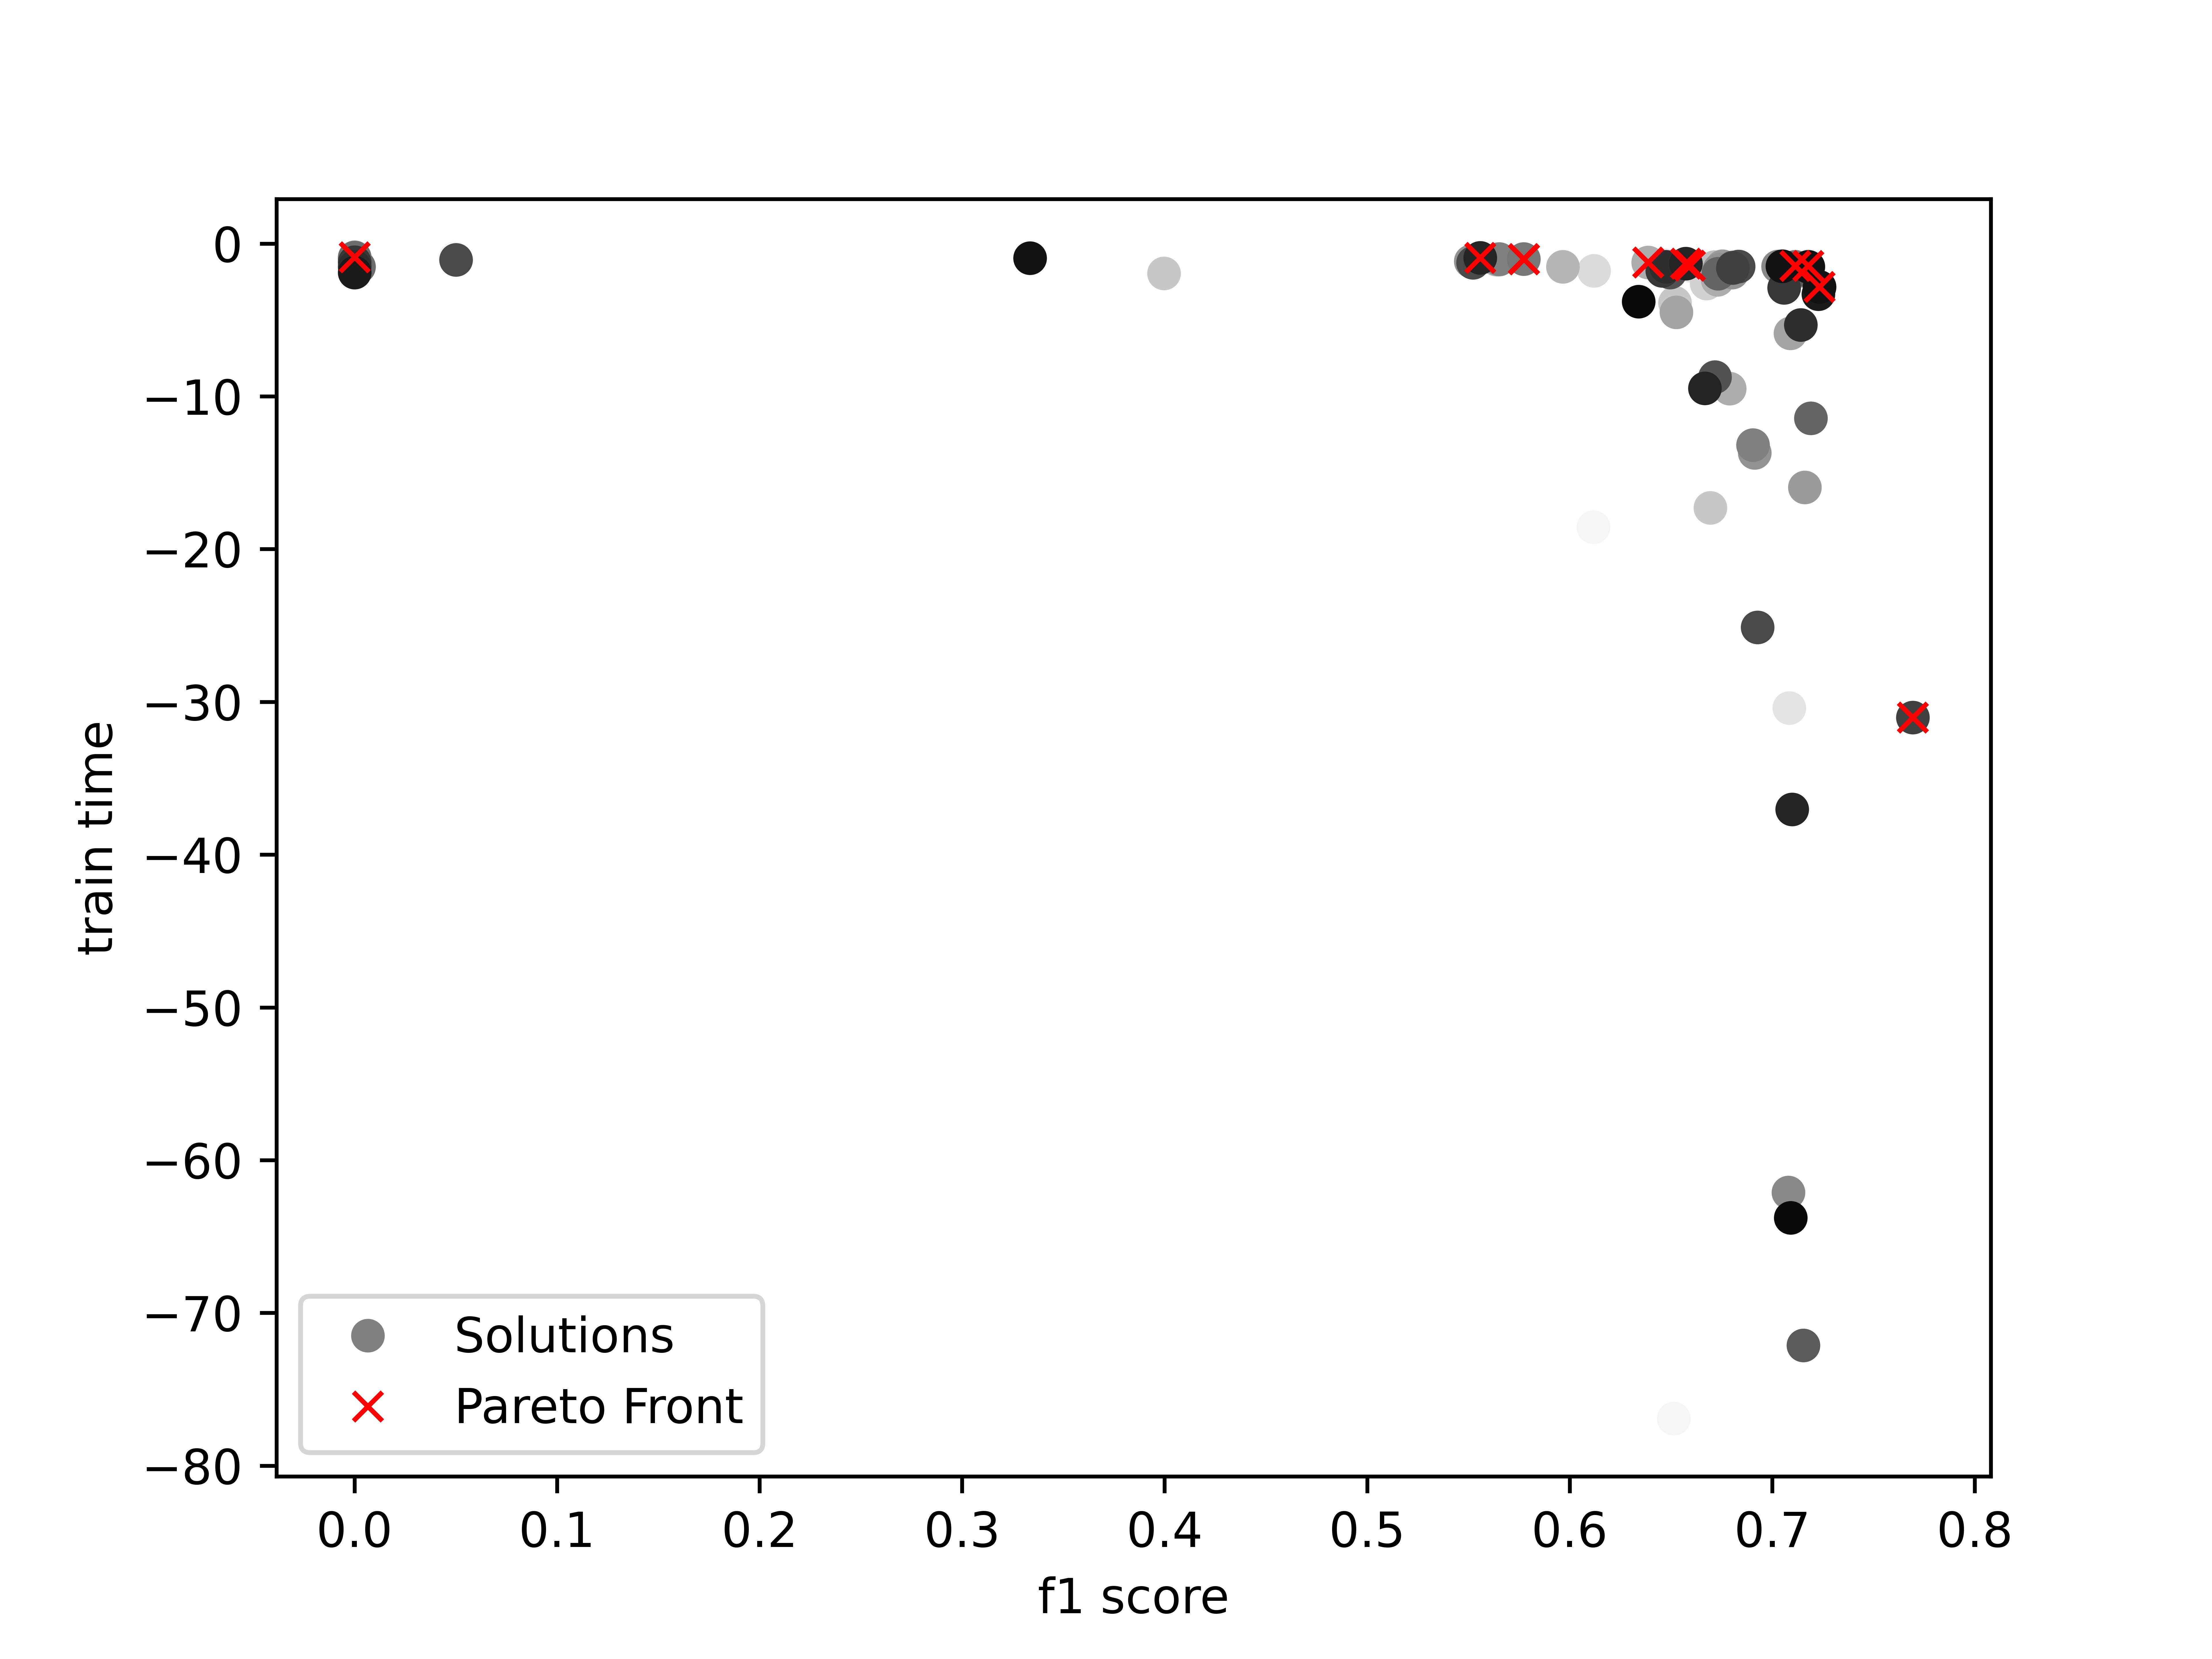
\includegraphics[scale=0.65]{Pictures/haha_fscore_vs_time_3min.jpg}
    \caption{HAHA: F-score contra Tiempo de Entrenamiento (3 minutos m\'ax)}
    \label{impl:fig:haha:fscore_vs_time_3min}
\end{figure}

\subsubsection{Precisi\'on contra Recobrado}
Contrario a lo que muestra la evaluaci\'on de Cars con respecto a precisi\'on y recobrado, durante esta prueba no es posible encontrar un flujo que maximice ambas m\'etricas y es necesario hacer concesiones entre una y la otra. El frente como se observa en la figura \ref{impl:fig:haha:precision_vs_recall} tiene una forma c\'onvexa, consecuencia del conflicto que se crea al optimizar para estas m\'etricas en este conjunto de datos.

\begin{figure}[ht]
    \centering
    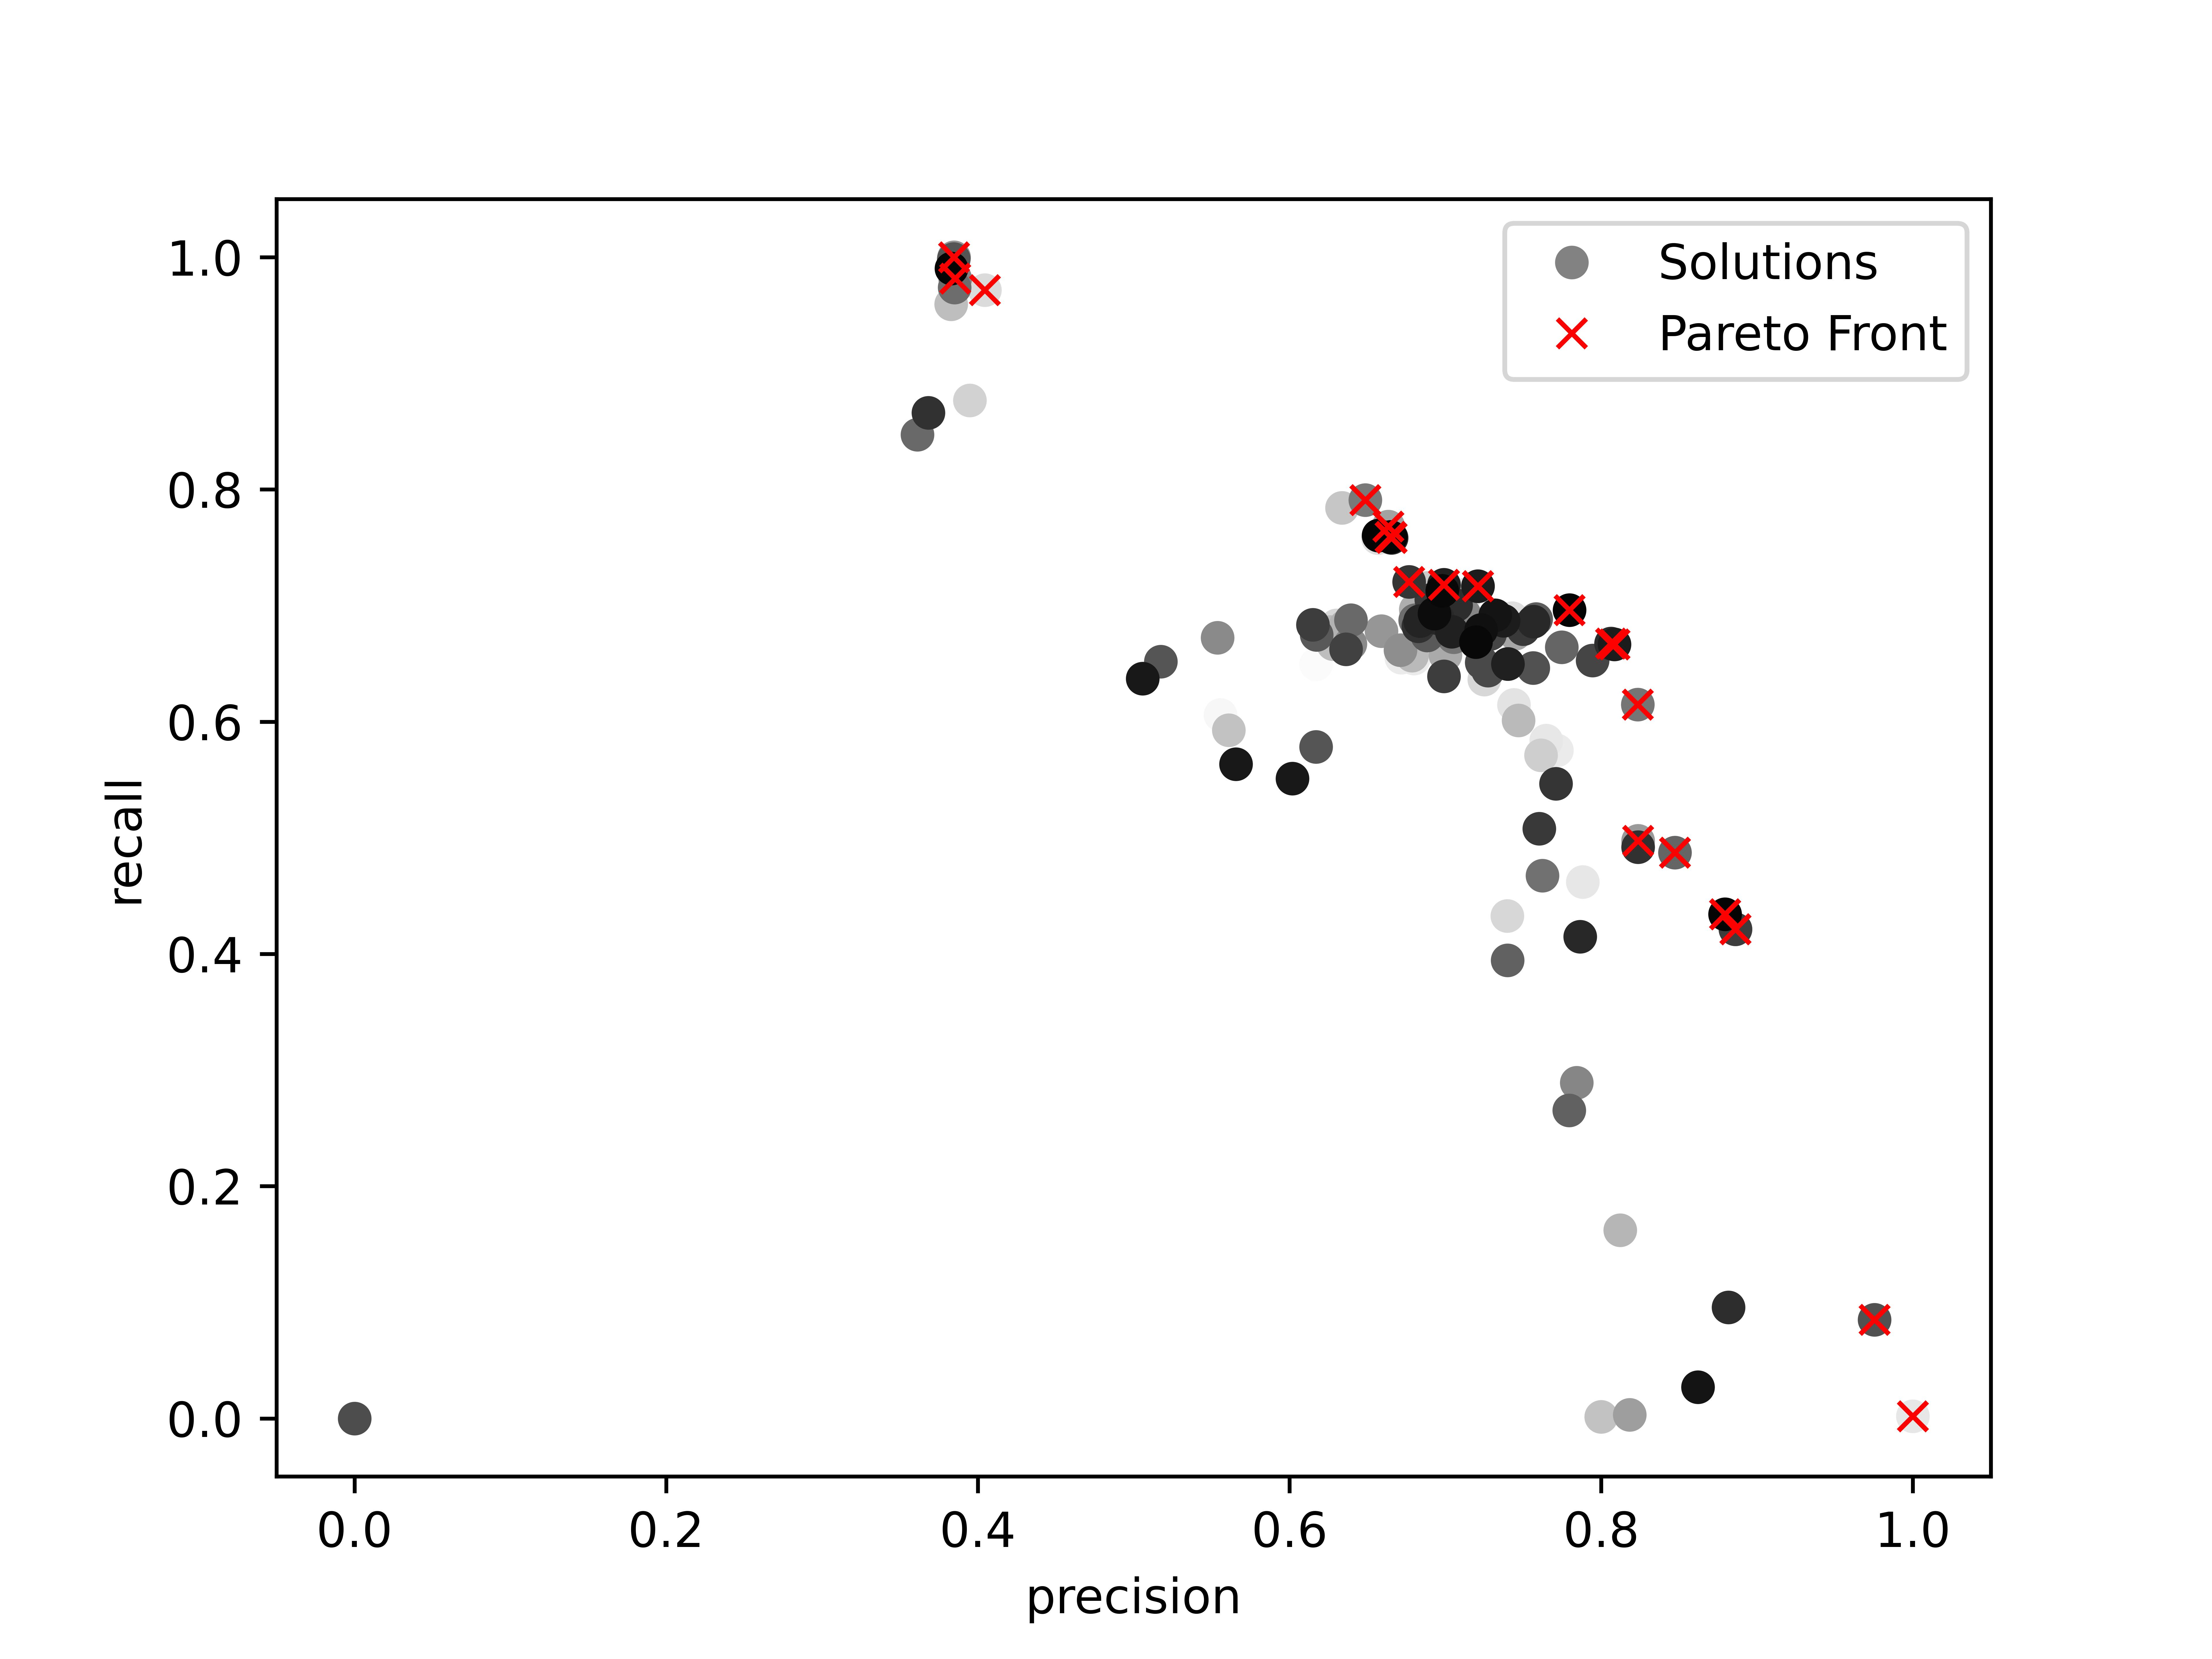
\includegraphics[scale=0.65]{Pictures/haha_precision_vs_recall.jpg}
    \caption{HAHA: Precisi\'on contra Recobrado (10 segundos m\'ax)}
    \label{impl:fig:haha:precision_vs_recall}
\end{figure}

Cuando se optimza con tiempo m\'aximo de tres minutos (ver figura \ref{impl:fig:haha:precision_vs_recall_3min}) no se muestra ning\'un cambio notable con respecto a la anterior prueba. 

\begin{figure}[ht]
    \centering
    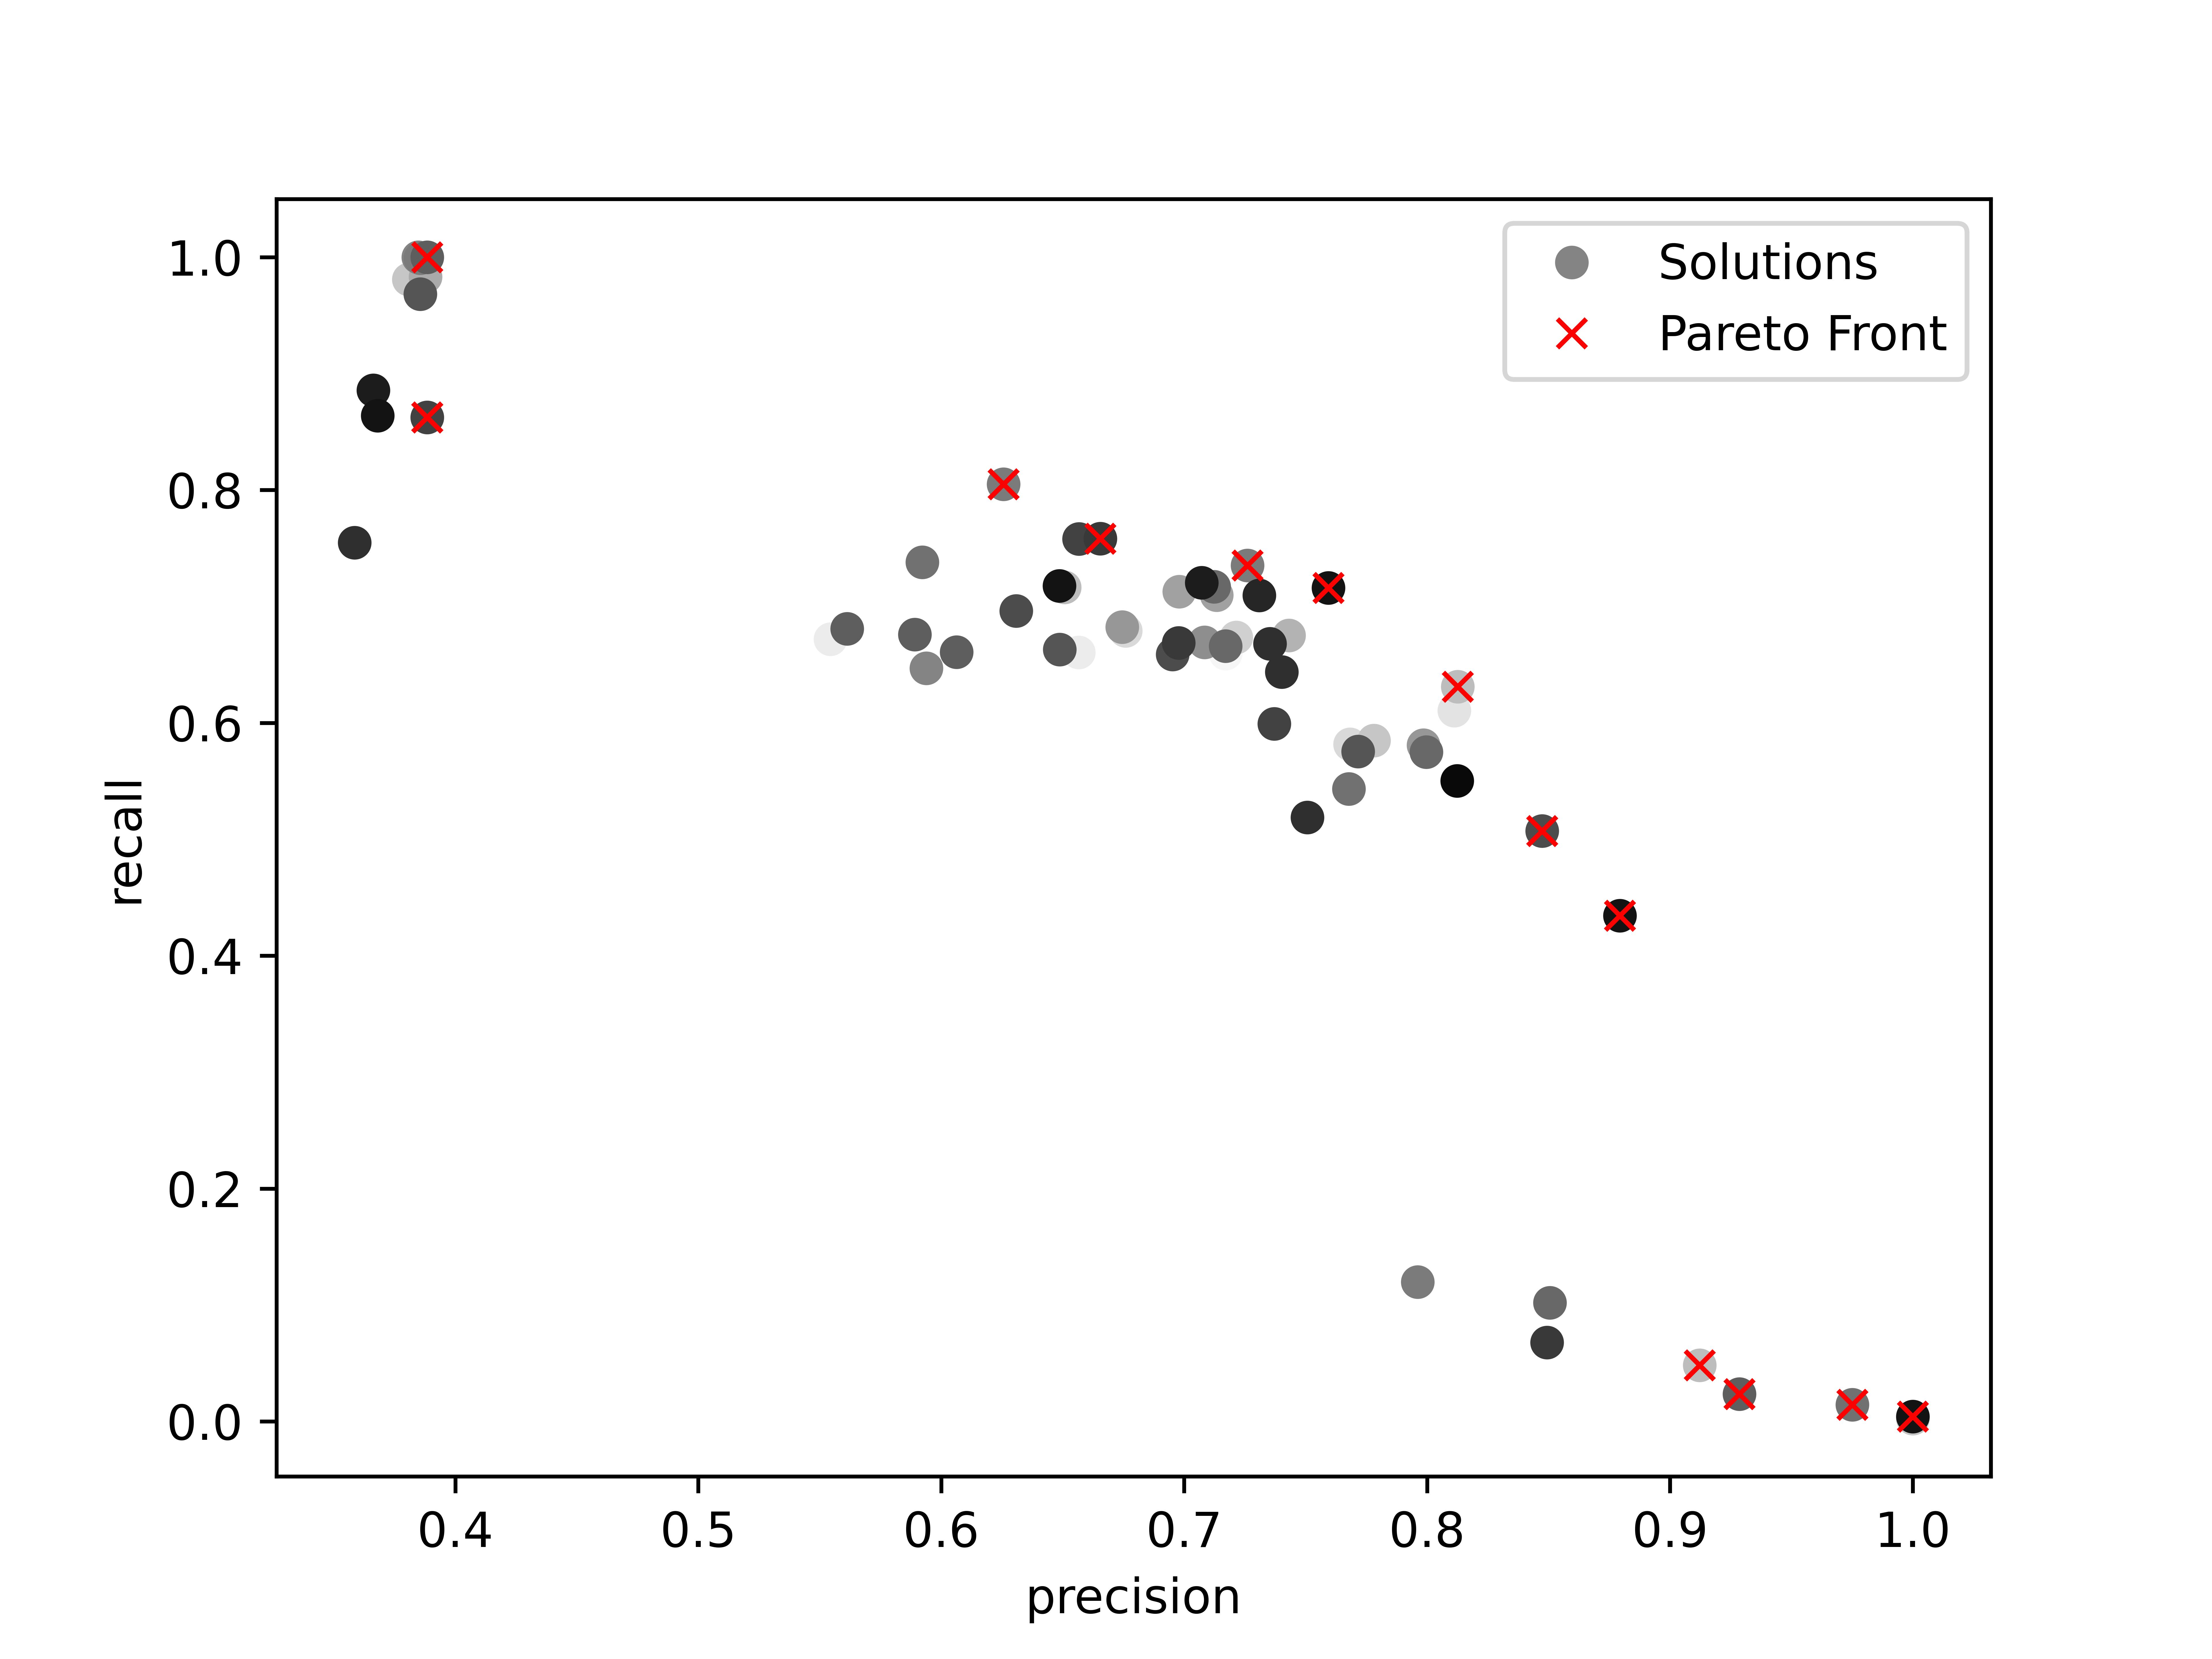
\includegraphics[scale=0.65]{Pictures/haha_precision_vs_recall_3min.jpg}
    \caption{HAHA: Precisi\'on contra Recobrado (3 minutos m\'ax)}
    \label{impl:fig:haha:precision_vs_recall_3min}
\end{figure}

\subsection{MEDDOCAN}
Este corpus representa el conjunto de datos m\'as grande de los tres y  fue necesario aumentar el tiempo de evaluaci\'on por flujo a 10 minutos con el fin de encontrar soluciones v\'alidas, estas tomando tiempes de entre 2 y 6 minutos. Las pruebas fueron ejecutadas con una poblaci\'on total de 50 individuos, 10 horas de tiempo m\'aximo y 10 minutos por evaluaci\'on. 
Las implementaciones de \textit{f-score}, precisi\'on y recobrado son las implementaciones del m\'odulo de Python \textit{meddocan}.
El entrenamiento en esta prueba resultaron ser m\'as lentos y no fue posible realizar muchas iteraciones por lo que no es posible apreciar completamente los frentes.
% Aqu\'i el tiempo m\'aximo es mucho mayor pues es un corpus es mucho m\'as grande que los anteriores que para encontrar al menos un pipeline v\'alido require alrededor de 7 u 8 minutos. Lo suficiente para lograr 3 o 4 generaciones de un total de 100.


\subsubsection{F-Score contra Tiempo de Entrenamiento}
En esta prueba se ve un comportamiento similar a las anteriores como puede observar en la figura  \ref{impl:fig:MEDDOCAN:fscore_vs_train_time} un poco m\'as acentuado en lo que se refiere a m\'etricas de tiempo de entrenamiento pues la diferencia pasa de ser de segundos a minutos. Existe una soluci\'on con un tiempo de 160 segundos y una precision de 0.83 contra una de 230 segundos y una precisi\'on cercana a 0.9.  

\begin{figure}[ht]
    \centering
    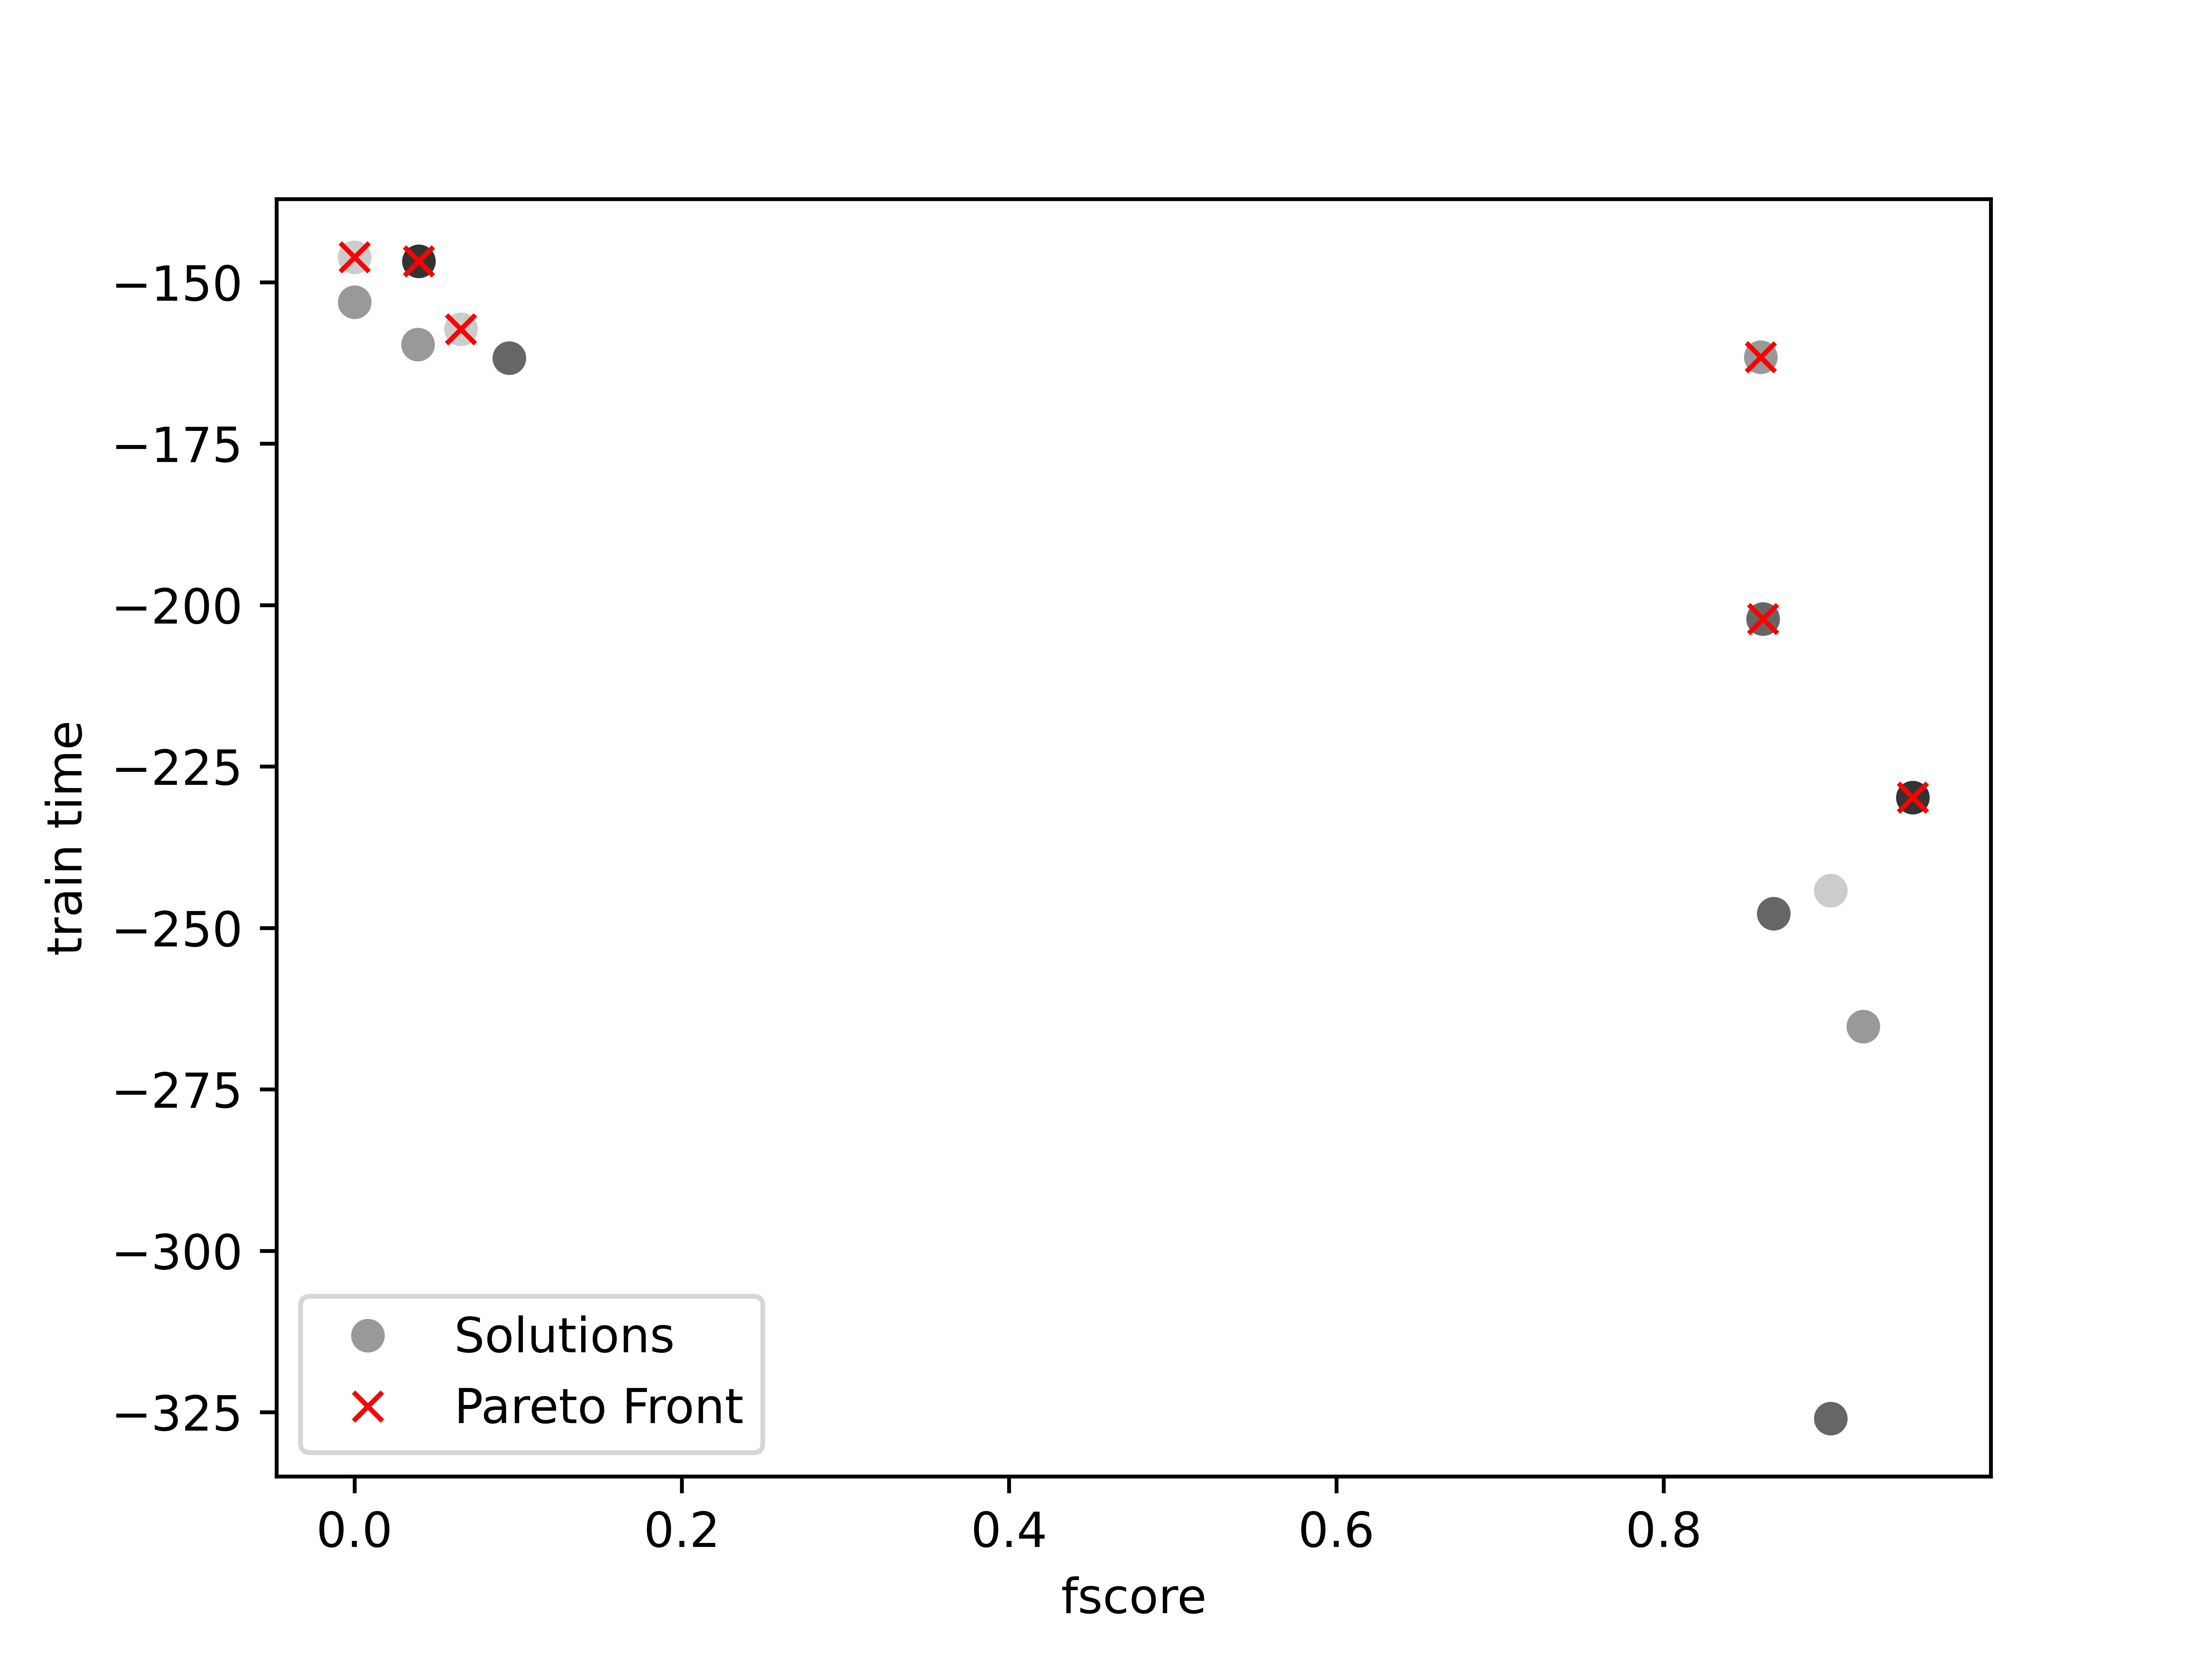
\includegraphics[scale=0.65]{Pictures/meddocan_fscore_vs_train.jpg}
    \caption{MEDDOCAN: F-Score contra Tiempo de Entrenamiento}
    \label{impl:fig:MEDDOCAN:fscore_vs_train_time}
\end{figure}


\subsubsection{Precisi\'on contra Recobrado}

En esta prueba, representada en la figura \ref{impl:fig:MEDDOCAN:precision_vs_recall}, debido a la poca cantiad de iteraciones se obtiene una representaci\'on muy probre del frente de Pareo. No queda claro si estamos frente a un caso parecido al de precisi\'on contra recobrado de Cars (\ref{impl:fig:cars:precision_vs_recall}) donde las m\'etricas no entran en conflicto y es posible optimizar para ambas, o mas parecido al caso en HAHA (\ref{impl:fig:haha:precision_vs_recall}) donde es obligatorio realizar concesiones.

Un dato interesante de esta prueba en comparaci\'on a cuando se optimiza \textit{f-score} contra tiempo de entrenamiento es que esta realizo menos iteraciones en el mismo rango de tiempo, visible por la diferencia de puntos graficados entre ambas. Esto sugiere que al optimizar utilizando el tiempo como una m\'etrica hace que el sistema priorize flujos r\'apidos de entrenar afectando positivamente la velocidad de b\'usqueda de AutoGOAL.

\begin{figure}[ht]
    \centering
    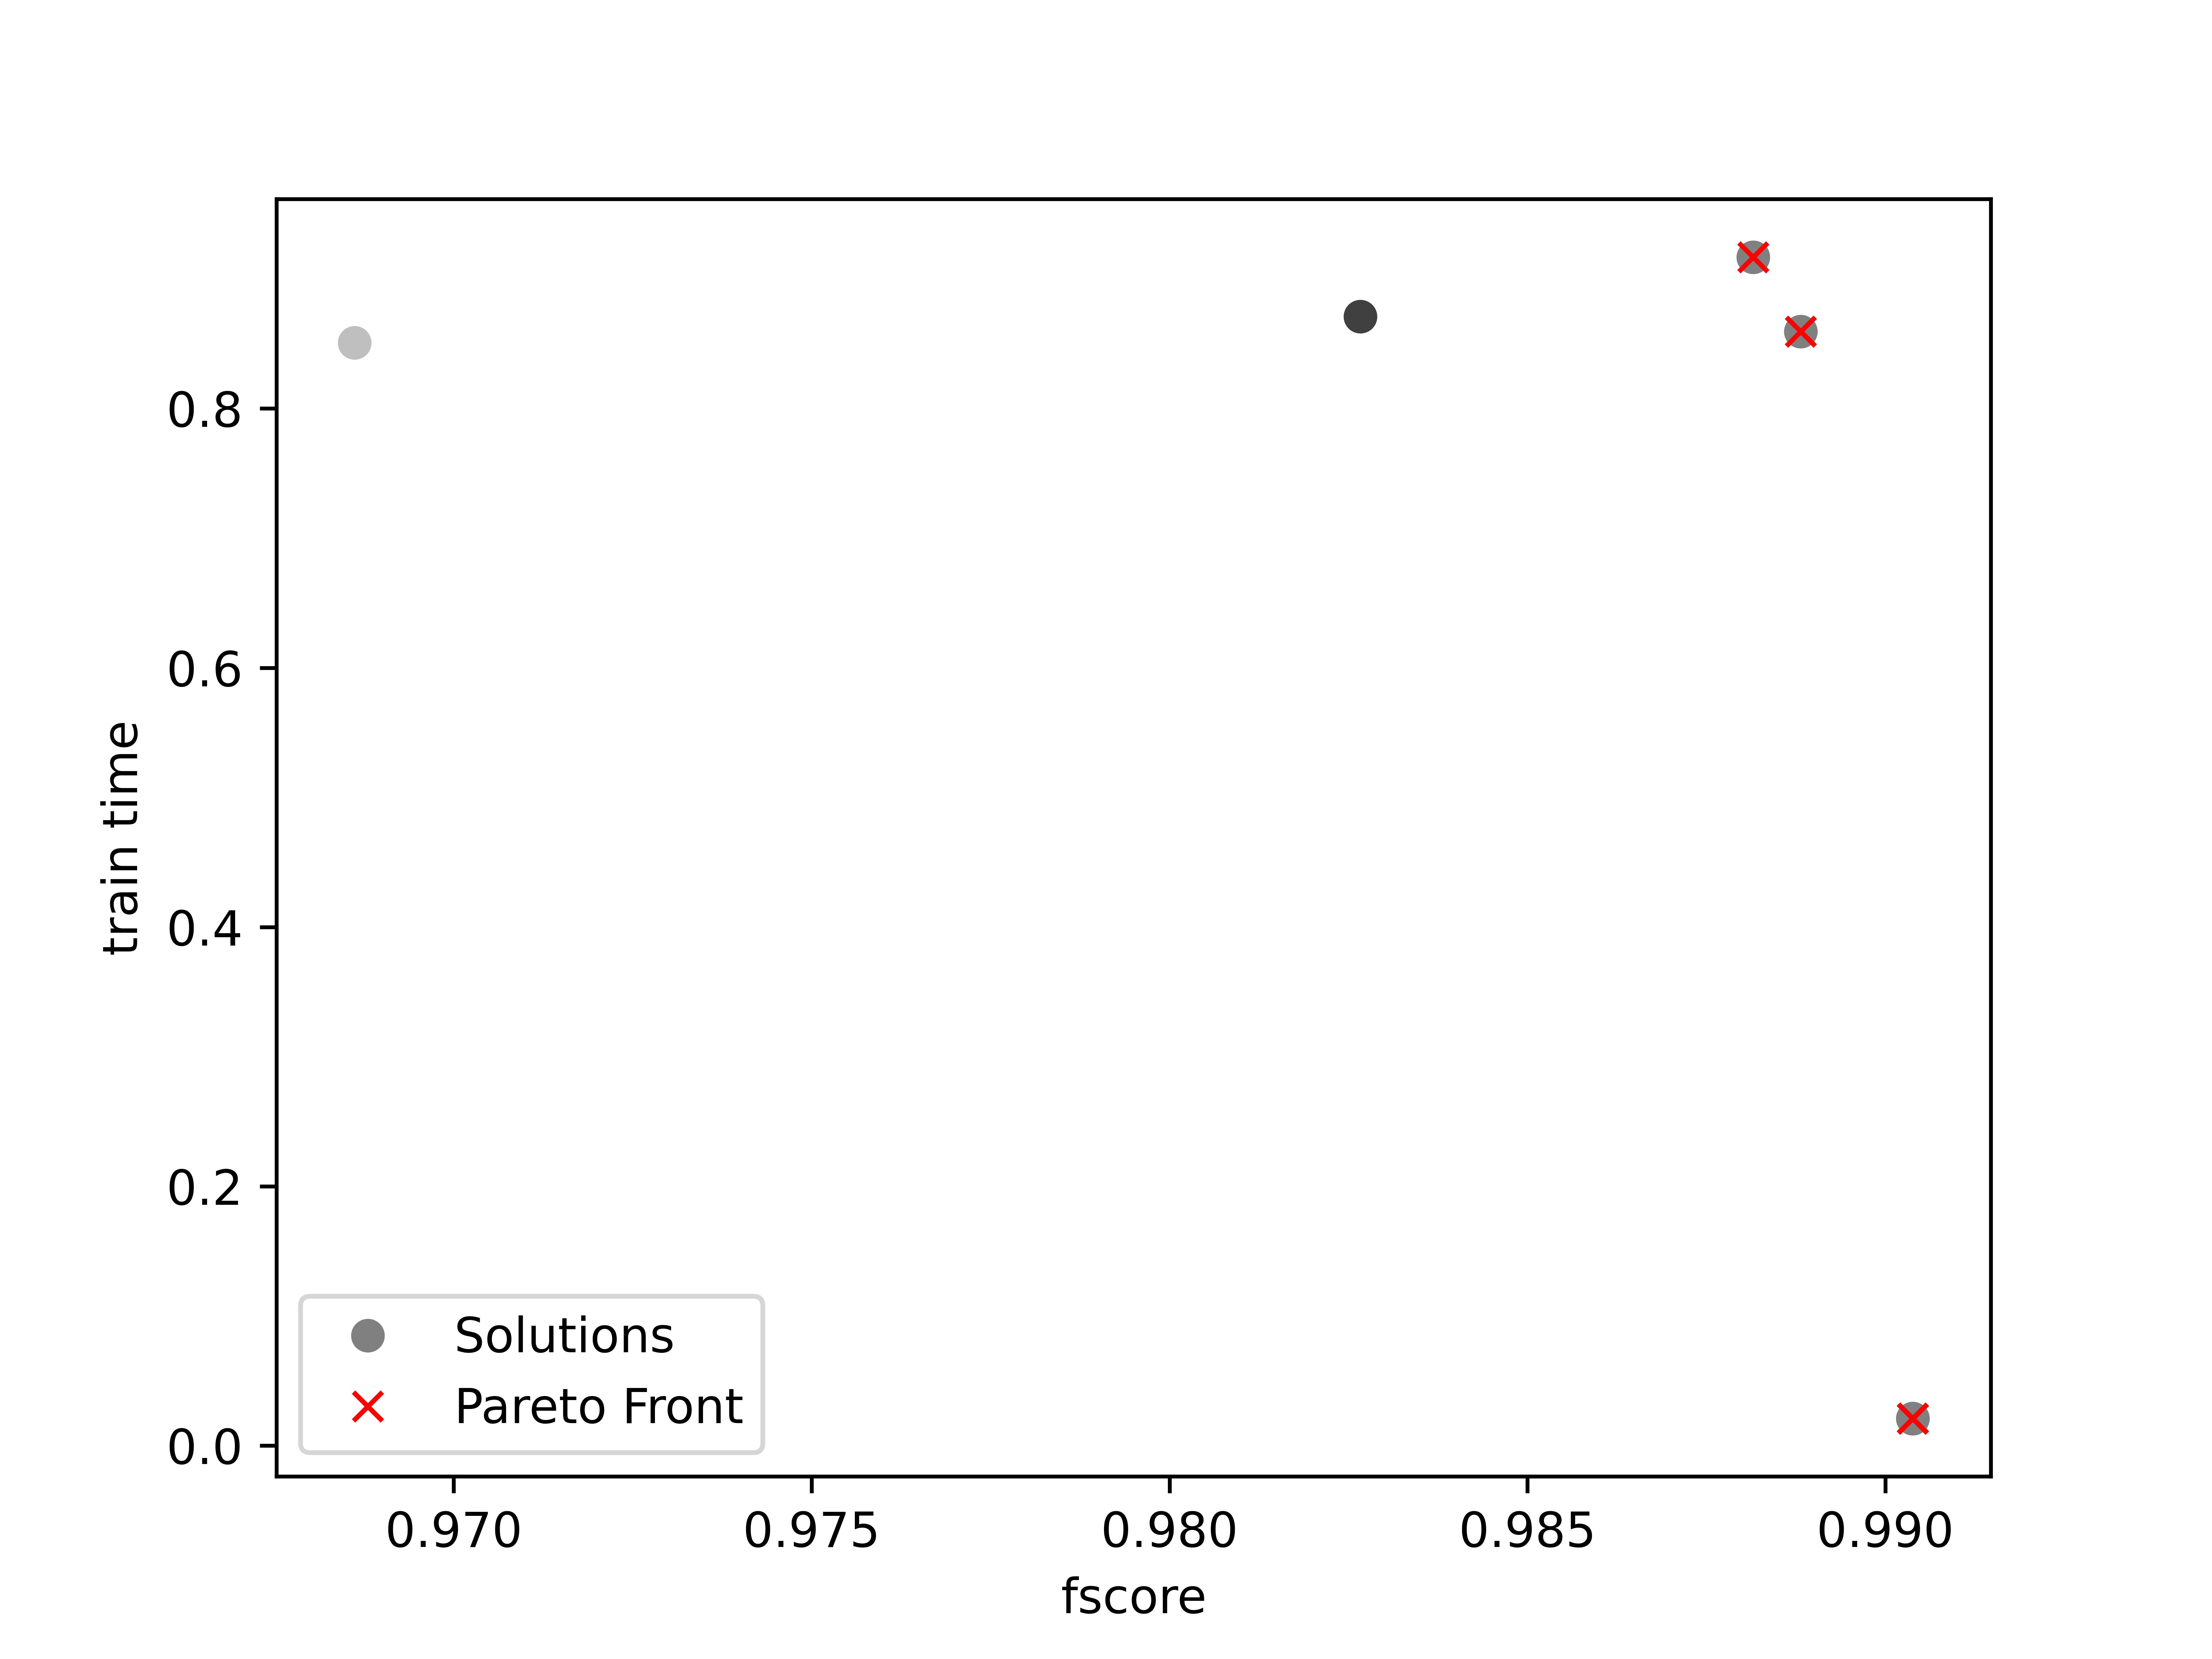
\includegraphics[scale=0.65]{Pictures/meddocan_precision_vs_recall.jpg}
    \caption{MEDDOCAN: Precisi\'on contra Recobrado}
    \label{impl:fig:MEDDOCAN:precision_vs_recall}
\end{figure}
